\section{Offset, Amplitude, Frequenz und Phase eines Pendels}

\subsection{Arbeitsgrundlagen}

\subsection{Durchf\"{u}hrung}

\subsubsection*{Versuchsanordnung}

\subsubsection*{Messergebnisse}

\begin{center}
    \begin{threeparttable}
        \caption{Gemessene Gr\"ossen}
        \begin{tabular}{*{12}{c}}
            \toprule
            $t(s)$  &  $y(m)$   &  $t(s)$   &  $y(m)$   &  $t(s)$  &  $y(m)$    &  $t(s)$   & $y(m)$    &  $t(s)$   &  $y(m)$   &  $t(m)$   &  $y(m)$ \\
            \midrule
            0.5     & -0.418    & 8.0       & 0.594     & 15.5     & -0.577     & 23.0      & 0.417     & 30.5      & -0.132    & 38.0      & 0.152   \\
            1.0     & -0.07     & 8.5       & 0.632     & 16.0     & -0.48      & 23.5      & 0.423     & 31.0      & -0.123    & 38.5      & 0.058   \\
            1.5     & 0.082     & 9.0       & 0.435     & 16.5     & -0.414     & 24.0      & 0.45      & 31.5      & -0.075    & 39.0      & 0.193   \\
            2.0     & 0.19      & 9.5       & 0.366     & 17.0     & -0.46      & 24.5      & 0.389     & 32.0      & -0.373    & 39.5      & 0.070   \\
            2.5     & 0.494     & 10        & 0.123     & 17.5     & -0.187     & 25.0      & 0.488     & 32.5      & -0.146    & 40.0      & 0.235   \\
            3.0     & 0.566     & 10.5      & 0.064     & 18.0     & -0.171     & 25.5      & 0.317     & 33.0      & -0.176    & 40.5      & 0.084   \\
            3.5     & 0.753     & 11.0      & -0.084    & 18.5     & -0.03      & 26.0      & 0.344     & 33.5      & -0.193    & 41.0      & 0.248   \\
            4.0     & 0.913     & 11.5      & -0.152    & 19.0     & -0.072     & 26.5      & 0.363     & 34.0      & -0.138    & 41.5      & 0.319   \\
            4.5     & 0.869     & 12.0      & -0.299    & 19.5     & -0.011     & 27.0      & 0.218     & 34.5      & -0.259    & 42.0      & 0.052   \\
            5.0     & 0.977     & 12.5      & -0.506    & 20.0     & 0.082      & 27.5      & 0.084     & 35.0      & -0.078    & 42.5      & 0.159   \\
            5.5     & 0.956     & 13.0      & -0.479    & 20.5     & 0.109      & 28.0      & 0.113     & 35.5      & 0.018     & 43.0      & 0.134   \\
            6.0     & 0.996     & 13.5      & -0.576    & 21.0     & 0.25       & 28.5      & 0.166     & 36.0      & -0.059    & 43.5      & 0.079   \\
            6.5     & 0.971     & 14.0      & -0.662    & 21.5     & 0.404      & 29.0      & 0.02      & 36.5      & 0.056     & 44.0      & 0.097   \\
            7.0     & 0.827     & 14.5      & -0.498    & 22.0     & 0.272      & 29.5      & -0.032    & 37.0      & 0.004     & 44.5      & 0.162   \\
            7.5     & 0.784     & 15.0      & -0.654    & 22.5     & 0.317      & 30.0      & 0.011     & 37.5      & 0.042     & 45.0      & 0.030   \\
            \bottomrule
        \end{tabular}
        \begin{tablenotes}
            \small
            \item \textbf{Hinweis:} Daten wurden vom Auftragsdokument kopiert.
        \end{tablenotes}
    \end{threeparttable}
\end{center}


\subsubsection*{QtiPlot}

\begin{figure}[H]
    \center
    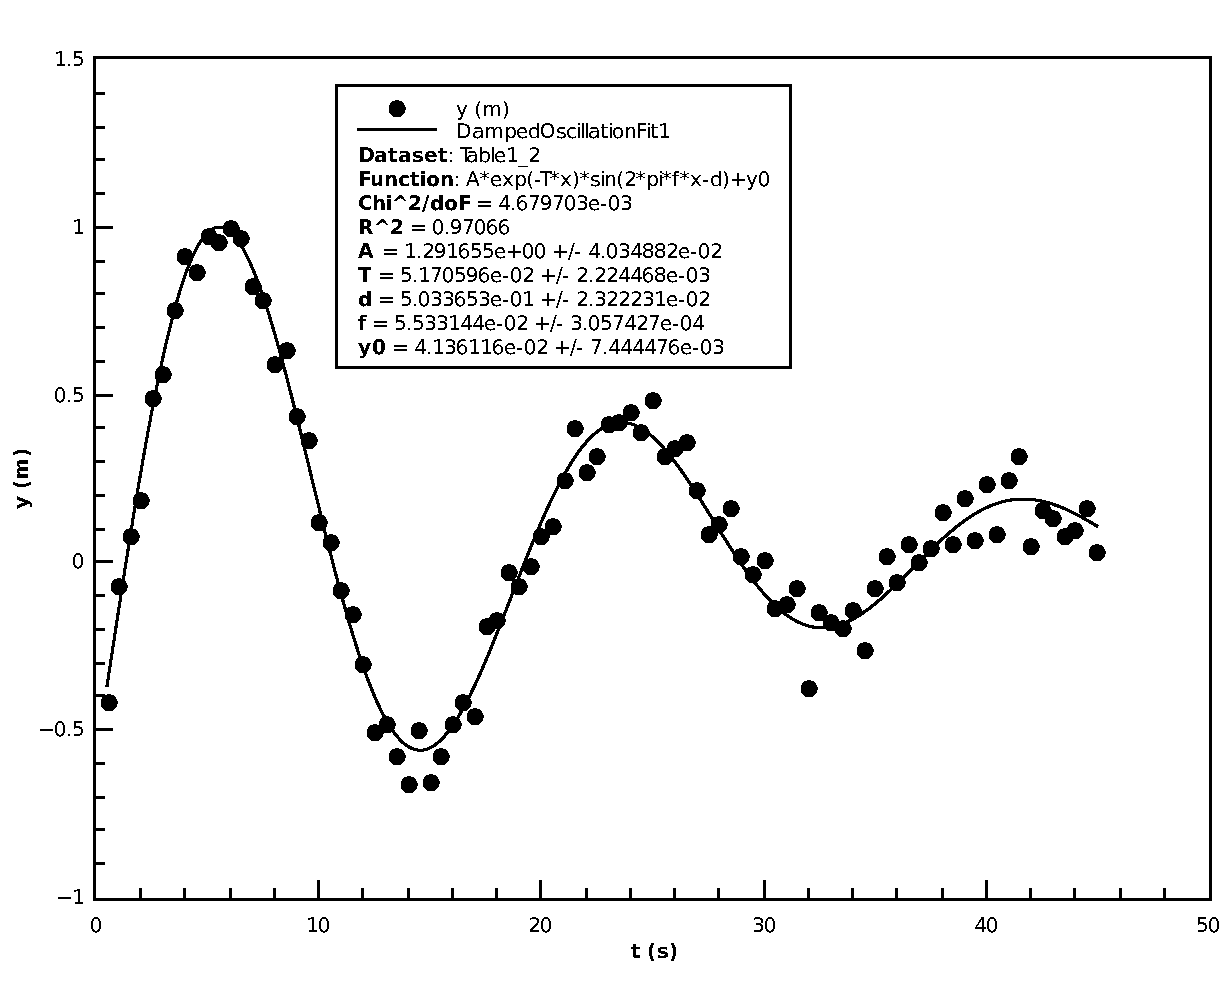
\includegraphics[width=.85\textwidth]{qtiplot/pendel}
    \caption{Nicht-lineare Regression zur Bestimmung von $A$, $\Gamma$, $f$, $\delta$ und $y0$}
    \label{fig:pendel}
\end{figure}

